\documentclass[a4paper, 12pt]{article}

\usepackage{graphicx}
\usepackage[margin=1in]{geometry}
\usepackage{amssymb}
\usepackage{comment}
\usepackage{amsmath}
\usepackage{setspace}

\begin{document}

	\pagenumbering{gobble}
	\title{Minimization of Time Required for Object in Free Fall to Reach Ground in Three Dimensional Space}
		\author{Nick Wang}
		\date{\today}
	\maketitle	
	
	\newpage
	\pagenumbering{roman}
	\tableofcontents

	\newpage
	\pagenumbering{arabic}
	\part{Interpretation of the problem}
		\section{Introduction}
		\paragraph
		\indent Imagine a squad of paratroopers about jump off a plane. Their goal is to reach an objective in the shortest amount of time possible. As the plane quickly approaches the objective, the paratroopers face a interesting question: what is the best time to jump?
		\paragraph
		\indent This is a similar scenario to popular video games of the battle royal genre, in which 100 players are dropped off a plane at the beginning of each round. The same question is asked by millions of players everyday, since being able to land earlier grants players a significant advantage, and an even more significant disadvantage to those landed late. As a gamer myself, I have spent many hours with friends yelling at my computer for loosing a game of battle royal, and hoped I could win more. At the time I first asked this question, I decided it is a trivial problem that would be naturally answered by experience. But after rounds and rounds, it came clear that while experience would certainly suffice the goal of not being the last to land, to be the first and gain an advantage, require a rigorous mathematical model to predict what is the best path to take to be the first landing. With this opportunity, I will attempt to solve this problem.
		\paragraph
		\indent A more methodical definition of this problem is given as follows:
		\subparagraph \indent An object moving in a three dimensional space, that is having three components to its displacement: x,y,z, is following a straight line. It is deciding at what time to deviate from its current path in order to move towards another point any where in the three dimensional space. To maximize its velocity or minimize its path in order to achieve the shortest time.
	
		\section{Mathematical reproduction of the problem}
		\paragraph \indent Furthermore, we must define the problem in strict mathematical terms:
		\subparagraph \indent As shown in the image below, a particle(plane), $P$, with a constant velocity vector $\vec{u} = <x_v,y_v,z_v>$, a point(objective) $O$, shown as a red point below, exists within  $\mathbb{R}^3$ at coordinate $O(x_o,y_o,z_o)$. The position of point $P$ is given as a parametric equation of $t$ where $\vec{s} = <x(t), y(t), z(t)>$, shown as a black vector in the image below. Another point $Q$ has position $\vec{r}$ and $\vec{r}=\vec{s} = <x(t), y(t), z(t)>, \{ t<k | k \subseteq \mathbb{R}$ and $k \geq 0 \}$. At $t=k$ point $Q$ changes its direction and obtains a new velocity $\vec{v} = <x(t), y(t), z(t)>$. The new  position of point $Q$ is $\vec{r_2} = <x(t), y(t), z(t)>$. Find the value of $k$ that minimizes the value of $t$ given the components of $\vec{u}$ and $O$.
		\begin{figure}[h!]
			\centering
				\centering
				 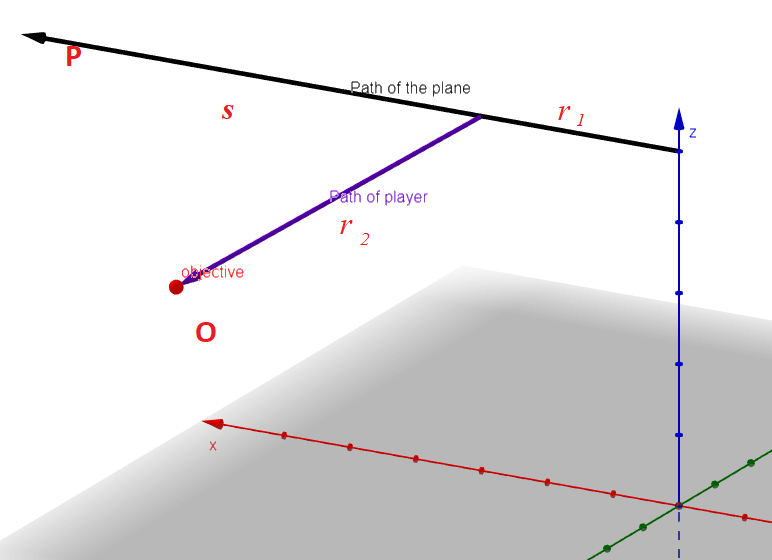
\includegraphics[width=.6\linewidth]{demonstration.png}
				 \caption{Demonstration of the problem}
		\end{figure}
		
		\paragraph
		\indent In order to find the minimal time it would take for the player to reach its objective, we must fist define the variables that would contribute to time. 
		\paragraph
		\indent First and foremost the path take by the player would have the greatest impact on time. We can easily see that velocity, another factor that determines time, is independent of the path chosen. Or in other words the path the player choose will not affect how fast he can go. Additionally it is also easy to see that the shorter the path, the shorter the time. Thus we conclude that:
		\subparagraph \indent The path that would lead to the shortest time is are straight line segments.
		\paragraph \indent The second factor that would contribute to time is the velocity. We can easily see that the particle $Q$ experiences 2 different velocities, $\vec{r}$ and $\vec{r_2}$. And since $\vec{r}$ a constant equal to $\vec{u}$, the only variable in this problem is $\vec{r_2}$. Thus naturally it may seem that the greater the magnitude of $\vec{r_2}$, the faster the particle will reach point $O$. But another crucial observation must be made to understand that because the particle is falling, its change in velocity, $\vec{a}$ equals to gravity. This would mean that the earlier the particle $Q$ deviates from the path of $P$, the greater the magnitude of $\vec{r_2}$. Then we make the conjecture that:
		\subparagraph \indent To minimize time we need to maximize the magnitude of $\vec{r_2}$.
		\paragraph \indent Based on the above 2 observations we can split the problem in to 2 stages, stage 1 and stage 2 as shown below. 
		\begin{figure}[h!]
			\centering
			\begin{minipage}{.5\textwidth}
				\centering
				 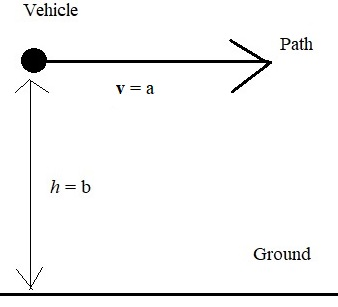
\includegraphics[width=.6\linewidth]{stage1.jpg}
				\caption{Stage 1}
			\end{minipage}%
			\begin{minipage}{.5\textwidth}
			\centering
				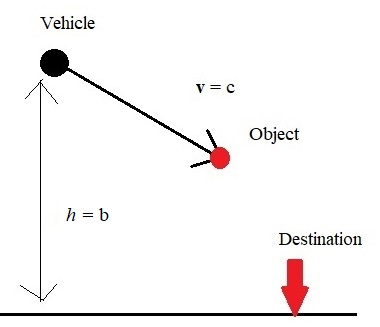
\includegraphics[width=.6\linewidth]{stage2.jpg}
				\caption{Stage 2}
			\end{minipage}
		\end{figure}
		\paragraph	
		\indent During stage 1 the path and velocity are constant, thus the duration of stage is only dependent on the time at which stage 2 begins, or the arbitrary time the player leaves the plane. Thus if stage 2 starts at $t=a$ , then the duration of stage 1 is $a$. Furthermore we can conclude that since velocity is constant, the time required to complete stage 1, $t_{stage1}$, is linear.
		\paragraph
		\indent Stage 2 consists of 2 sub-stages, first sub-stage is when the player is first thrown off the plane and is in a controlled free fall. During this stage the velocity will increase with $\vec{a} = <0,0,-9.8>$. The second sub-stage is when the player reach a certain altitude and opens its parachute, which will slow this player to a constant speed.
		\paragraph
		\indent Based on these observations, the following equation of $T_{total}$ at a point $R$ where $t_{stage1}$ and $t_{stage2}$ are known can be deduced: $$T_{total} = t_{stage1} + t_{stage2}$$ Thus $T_{total}$ at another point can also be deduced in relation to point $R$: $$T_{total2} = t_{stage1} + \Delta t_{stage1} + t_{stage2}+\Delta t_{stage2}$$ That $T_{total2}$ is the sum of $T_{total}$ at point $P$ and the difference in duration of $t_{stage1}$ and the difference in duration of $t_{stage2}$. And the desire is that $T_{total2} < T_{total}$, thus: $$T_{total2} - T_{total} \leq 0$$
		$$ t_{stage1} + \Delta t_{stage1} + t_{stage2}+\Delta t_{stage2} - t_{stage1} - t_{stage2} \leq 0$$
		$$ \Delta t_{stage1} + \Delta t_{stage2} \leq 0$$
		This inequality will be further examined in later discussions.

		\section{Assumptions and definitions}
		\paragraph
		\indent The combination of the two stages produce a simplified mathematical representation of the problem. But with further thought we would realize that this representation avoided consideration of factors such as air resistance and terminal velocity.
		\paragraph
		\indent Thus we will impose the following restrictions:
		\begin{enumerate}
			\item[-] Air resistance: Air resistance will be ignored.
			\item[-] Terminal velocity: The falling object will reach an arbitrarily defined terminal velocity, and keep falling at this velocity in sub-stage 1 until sub-stage 2 is reached.
		\end{enumerate}
		\paragraph
		\indent The final stages of the fall, after the parachute is released, the player experiences a limited period of deceleration. This period of time, again, is independent of the height of the fall, and is completely arbitrary. Mathematically one can describe this as:
		$$T_{total} = (H_{total}-h_{final})/V_{total} + h_{final}/v_{final}$$\\
		\indent	\indent \textit{Where:}\\
		\begin{center}
		 $H \equiv height$\\
		 $v \equiv velocity$\\
		\end{center}
		\paragraph \indent Since $h_{final}$ is an arbitrary constant, can be substituted with constant $c$.\\
		\indent \indent Thus
		\begin{center}
			$$\lim_{H\to\infty} t_{final}/T_{total} = c/v_{final} / (H_{total}-c)/V_{total}$$
			$$ \lim_{H\to\infty} t_{final}/T_{total} = \frac{c}{v_{final}}/\frac{(H_{total}-c)}{v_{total}}$$
			$$ \lim_{H\to\infty} t_{final}/T_{total} = 0 $$
		\end{center}
		\paragraph
		\indent Thus the duration of the final stages is negligible, thus it is safe to ignore this stage.
		\paragraph
		\indent With the above restriction we have greatly simplify the problem into its essence. This indeed will undoubtedly reduce the accuracy of our results, but we hope the discrepancy is negligible.

	\part{Additional Observations and Speculations}
		\section{Speculations}
		\paragraph
		\indent With the problem and variables defined, we will now look at the problem as a whole and provide some speculations. As explained in Part I Mathematical Reproduction of the Problem, the overall time is the duration of stage 1 and 2 combined, and the aim is to minimize this sum. Of these two stages it is easy to see that stage 2 is symmetrical to the normal line to the path of the plane that passes through the destination point as shown in figure 4.
		\begin{figure}[h]
			\centering
			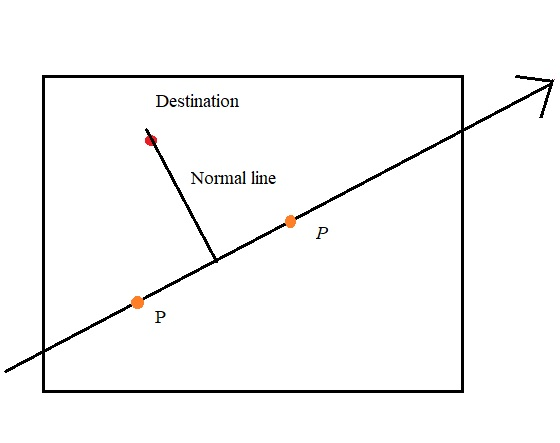
\includegraphics[width=0.6\textwidth]{Symmetry.jpg}
			\caption{Symmetry about normal line}
		\end{figure}
		\paragraph This is an important observation since under the current conditions we are modeling the optimal solution based on the distance of the path. This can be easily proven because:
		\begin{enumerate}
			\item[1] There is only one shortest distance from a fixed plane path and a destination point, $D$.
			\item[2] If we set the distance from the point $B$ as shown above to the intersect of the normal line and the plane's path to $l$, the distance between our destination and plane's path to $m$ and the height to be $h$, it is not hard to see:
			\begin{center}
						$$min(\vert DB \vert) = \sqrt{l^2 + m^2 + h^2} $$
			\end{center}
		\end{enumerate}
		\paragraph
		\indent Since this distance is identical at either B or \textit{B}, the duration of stage 2 at any point after the plane crosses the normal line has an identical, symmetrical point before the plane passes through the normal line. Thus the time it would take to complete stage 2 with either path shown in Figure 4 is the same, at the same time the time it would take to travel from $B$ to \textit{B} would be positive. Thus $T_{total1}$ at point $B$ compared to $T_{total2}$ at point \textit{B} is:
		\begin{center}
		$$\because T_{total2} = t_{stage1} + \Delta t_{stage1} + t_{stage2}+\Delta t_{stage2}$$
		$$\because \Delta t_{stage2} = 0$$
		$$\therefore T_{total2} = t_{stage1} + \Delta t_{stage1} + t_{stage2}$$
		$$\because \Delta t_{stage1} > 0$$
		$$\therefore min(T_{total1}) < min(T_{total2})$$
		\end{center}				
		Thus we can conclude that for any $t$ where the plane has passed the intersection of the plane's path and the normal line  $t$ cannot be at its minimum value, thus we can apply a upper bound to the value of $k$. 
		\paragraph
		\indent A further speculation can be made that the furthest distance the player can reach is a radius around the point where the player leaves the plane as shown in figure 5, and this radius is limited. Thus if the player leaves the plane way too early, or from a mathematical perspective, as the beginning time of stage 2 shifts further towards negative infinity, the player will never reach the desired location. Thus we can conclude that one mustn't leave the plane too early.
		\begin{figure}[h!]
			\centering
			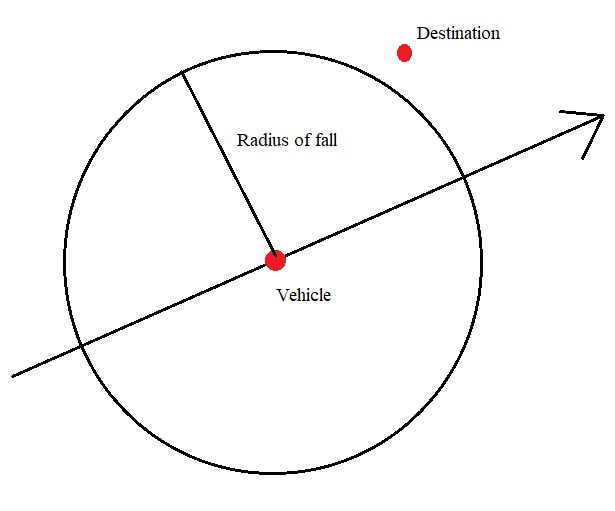
\includegraphics[width=0.6\textwidth]{Radius.jpg}
			\caption{Radius of reach}
		\end{figure}
		\\Thus it can be further deduced that the duration of stage 1 is
		 $$t_{stage1} \leq t_{enteringMaxRadius}$$

	\part{Calculations}
		\paragraph
		\indent Now we can move on to finding a solution. Since the original problem is given in symbolic terms, we will assign arbitrary values to these variables to obtain a numerical solution. So the new problem as follows:
		\subparagraph \indent A plane, $P$, with a velocity vector $\vec{u} = <300,0,0>$ flying from the $z$-axis at constant height $z=5000$. The objective $O$, lies on the $xy$-axis at coordinate $O(3000,1000,0)$. The position of point $P$ is given as a parametric equation of $t$ where $\vec{s} = <x(t), y(t), z(t)>$. A parachuter $Q$ has position $\vec{r}$ and $\vec{r}=\vec{s} = <x(t), y(t), z(t)>, \{ t<k | k \subseteq \mathbb{R}$ and $ k \geq 0 \}$. At $t=k$ the parachuter jumps off the plane. Find the $k$ value that minimizes the value of $t$ when the parachuter reaches the point $O$
		
		Thus we need to first obtain the position vector of the plane.
		$$\vec{s} = \int \vec{u} dt$$
		$$\vec{s} = \int <300,0,0>$$
		$$\vec{s} = <\int 300 dt,\int 0 dt,\int 0 dt>$$
		$$\vec{s} = <300t+c_1,c_2,c_3>$$
		Since an initial position is given, we substitute in values to solve for $c_1,c_2, and c_3$
		$$\vec{s}(0) = <300\cdot 0 + c_1,c_2,c_3>$$
		$$<0,0,5000> = <300\cdot 0 + c_1,c_2,c_3>$$
		$$<c_1, c_2, c_3> = <0,0,5000>$$
		$$\vec{s}(0) = <300t,0,5000>$$
		Then we need to obtain the position vector of the parachuter after jumping off the plane,$\vec{r}$:
		$$\vec{r}' = \int \vec{s}'' dt_2$$
		$$\vec{r}'' = <0,0,-9.8>$$ 
		$$\vec{r}' = <\int 0 dt_2, \int 0 dt_2,\int -9.8 dt_2>$$
		$$\vec{r}' = <c_1, c_2,-9.8\cdot t_2 +c_3>$$
		Since the parachuter moves along the plane before jumping off, it initial velocity $\vec{r}'(k) = \vec{s}(k) = <300,0,0>$. And an important distinction that needs to be made is that $t_2$ in the equation is not the same as $t$, since $t_2$ is the time after the parachuter jumps off the plane. Thus we must substitute $t_2$ with $t = t_2 + k$. Also when the parachuter jumps off the plane it obtains a initial velocity of 5 meter/second along the $y$-axis. Thus we have 
		$$\vec{r}' = <c_1, c_2,-9.8\cdot (t-k) +c_3>$$
		Now solving for $c$s
		$$\vec{r}'(k) = <c_1, c_2,-9.8\cdot (k-k) +c_3>$$
		$$<300,5,0> = <c_1, c_2,-9.8\cdot (k-k) +c_3>$$
		$$<c_1, c_2, c_3> = <300,5,0>$$
		$$\vec{r}' = <300, 5,-9.8\cdot (t-k)>$$
		Thus the position is:
		$$\vec{r} = \int \vec{s}' dt_3$$
		$$\vec{r} = \int <300, 5,-9.8\cdot (t-k)>dt_3$$
		$$\vec{r} = <\int 300 dt_3, \int 5 dt_3,\int -9.8\cdot (t-k) dt_3>$$
		$$\vec{r} = <300t +c_1, 5t + c_2, -9.8\cdot (t-k)^2+c_3>$$
		For the same reason $t_2$ is substituted with $t-k$, the velocity in the $y$-axis direction is only after the parachuter jumped out of the plane, we substitute $t_3$ of $y$-component with $t_3 = t-k$ and have:
		$$\vec{r} = <300t +c_1, 5(t-k) + c_2, -9.8\cdot (t-k)^2+c_2>$$
		Now acquiring the initial position. Since the initial position of the parachuter also travels along the plane:
		$$\vec{r}(k) =\vec{s}(0) = <300t,0,5000>$$
		$$\vec{r}(k) =\vec{s}(0) = <300k,0,5000>$$
		Solving for $c$s:
		$$\vec{r}(k) = <300k +c_1, 5(t-k) + c_2, -9.8\cdot (k-k)^2+c_3>$$
		$$<300k,0,5000> = <300k +c_1, 5(k-k) + c_2, -9.8\cdot (k-k)^2+c_3>$$
		$$<c_1, c_2, c_3> = <0,0,5000>$$
		Thus the position vector for the parachuter is:
		\begin{equation}
 			\vec{r} = \begin{cases}
  			<300t,0,5000>  & 0 < t < k \\
 			<300k , 5(t-k), -9.8\cdot (t-k)^2+5000>                                       & t \geq k
  			\end{cases} \\
		\end{equation}
		
		\paragraph \indent At this point, it became incredibly difficult to find the minimum value of $t$ since now it involves differentiation of parametric equations with multiple variables. To continue the above approach, I need a better understanding of multivariate and vector calculus. Thus a different approach might be taken. From now on we will look at a more geometrical interpretation of this problem.
		\paragraph \indent To move on, we need to look back at the inequality we derived in Part I: $$ \Delta t_{stage1} + \Delta t_{stage2} \leq 0$$
		Which describes the relation between the change of $t_{stage1}$ and the change of $t_{stage} 2$. Since in this case we only care about how rapidly these two values change, or in other words, we want to know at which point does the rate of change of $t_{stage1}$ equals the rate of change of $t_{stage} 2$, the change in $t$ can be interpreted as the derivative of $t$.\\ 
		Thus we have:
		$$ dt_{stage1} + dt_{stage2} \leq 0$$
		Since the duration of stage 1 is linear as discussed above, thus the change in duration of stage 1 is a constant:$$\frac{d}{dT_{total}}t_{stage1} = 1 $$
		Thus the inequality can be rewritten as: $$1 + dt_{stage2} \leq 0$$
		$$1 \leq -dt_{stage2}$$
		$$dt_{stage2} \leq -1$$
		\paragraph
		\indent To elaborate on this new inequality, as the plane moves along the path, the duration of stage 2 is decreasing. But there will be a point where they amount of duration that would be decreases if the player remained on the plane is less than the increase of duration of stage 1 by remaining on the plane. Thus by finding this point where $dt_{stage2} > -1$, we find the optimal position to leave the plane.
		\begin{figure}[h!]
			\centering
			 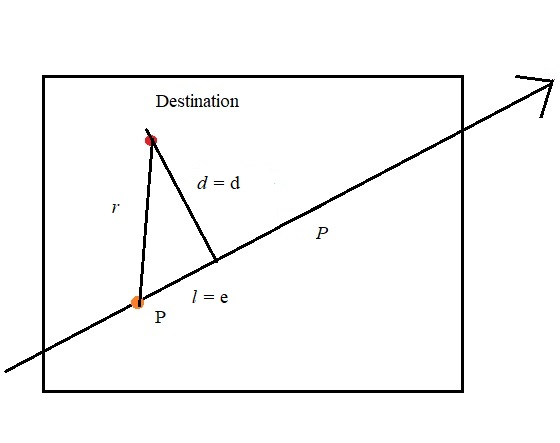
\includegraphics[width=.6\linewidth]{distance.jpg}
			\caption{The horizontal distance, r, the player has to travel}
			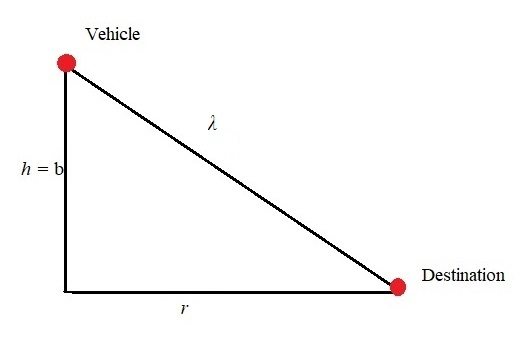
\includegraphics[width=.6\linewidth]{duration.jpg}
			\caption{The total distance, $\lambda$ , the player has to travel}
		\end{figure}
		\paragraph
		\indent To calculate the total distance as shown in figure 6, $d$ would be given since it can be measured as the distance between the destination and the path. We also need to know what the value of $l$ is, and as we've established, the point K is where stage 1 ends, and stage 1 is bounded in $t_{maxRadius} \geq t_{stage1} \geq t_{crossing}$. Thus we can define t as time before reaching the normal line, and $l = t\cdot v$, where $v$ is the velocity of the plane, and: $$r=\sqrt{(tv)^2+d^2}$$
		Referring to figure 7, we can see that $\lambda$ is dependent upon $h$, which is a constant that would be known is a specific example, and $r$, which was just calculated. Thus $$\lambda = \sqrt{b^2+r^2}$$
		Substituting in $r$: $$\lambda = \sqrt{b^2+\sqrt{(tv)^2 + d^2}^2}$$
		Simplifying: $$\lambda = \sqrt{b^2 + (tv)^2 + d^2}$$
		Because $b,v,d$ are all constants, we can take them out and replace them with another constant, where $\alpha = v^2$, $\beta = b^2 + d^2$: $$\lambda = \sqrt{\alpha t^2 + \beta}$$
		At this point, we need to take in to consideration of another variable, terminal velocity.\\
		Terminal velocity is obtained after a certain amount of time an object is in free fall when gravitational acceleration is canceled out by the air resistance and stops to accelerate. This would complicate the problem by a great deal, thus we will ignore the acceleration stage of the parachuter, and he will immediately reach terminal velocity the instant he jumps out of the plane. This can be justified by the same reason we have chosen to ignore the final deceleration stage in Part I, where we concluded that the impact of deceleration on total time is negligible. And in reality the distance one has to fall is also proven to be so, about 450 meters, a small distance compared to the 5000 meter of the problem.\\
		Since the player falls at a constant terminal velocity, thus $t_{stage2} = \frac{\lambda}{v_{terminal}}$, and $v_{terminal}$ is arbitrarily defined.
		Substituting in $\lambda$: $$ \frac{ \sqrt{\alpha t^2 + \beta}}{v_{terminal}}$$
		Simplifying: $$\lambda = \gamma \sqrt{\alpha t^2 + \beta}, where \gamma = \frac{1}{v_{terminal}}$$
		Taking derivative of $k$: $$\lambda' = 2 \alpha t{( \alpha t^2 + \beta )}^{-1/2}$$
		Thus plugging back into the inequality: $$2 \alpha t {( \alpha t^2 + \beta )}^{-1/2} = -1$$
		Thus we substitute in the given condition to solve for t:
		$$2\cdot 300^2 \cdot t(300^2 \cdot t^2 + (5000^2 + 1000^2))^{-\frac{1}{2}}+1 = 0 $$
		We solve for it graphically:
		\begin{figure}[h!]
			\centering
			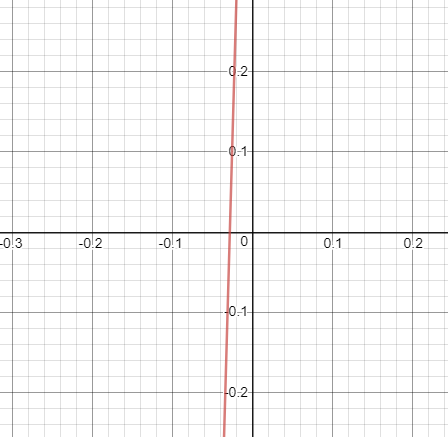
\includegraphics[width=0.4\textwidth]{solution.PNG}
			\caption{Graphical Solution}
		\end{figure}
		\\We arrive at an answer of $t=-0.0283 seconds$, or 0.0283 seconds before reaching the intersection between the plane's path and the normal line between the destination and plane's path.
	\part{Conclusion}
		\section{Conclusion}
		\paragraph
		\indent The solution of $t=-0.0283$ suggests that on a grand scale should jump a fraction of a second before the plane reaches the point on its path that is the shortest to the destination. It means that the effect of jumping off the plane early has essentially no effect on the time it would take for the parachuter to reach its destination. This would mean that the parachuter's component speeds are way too small compared to the velocity of the plane, and it is best to wait on the plane, and jump the moment the plane reached the shortest point described above.
		\paragraph
		\indent But on the other hand, if the plane travels at a significantly slower speed and on a significantly smaller scale, jumping early would have a much bigger impact. In a different scenario where the plane travels at 2 meters/second and the distance the parachuter has to travel is only 1000 meter horizontally and 1000 meter vertically, he should jump 3 minutes before the plane reaches the shortest distance point, according to the same equation. This would better fit the description of the video games mentioned in the introduction of the problem.
		\paragraph
		\indent Overall, the simpler geometric interpretation of this problem yielded  reasonable result. But due to its many assumptions and simplifications, one do not know the true accuracy of this model. But one thing is certain, if the vector method can be continued, it would have yielded a more accurate result, while requiring much deeper knowledge of Calculus.
		
		\newpage
		\begin{thebibliography}{9}
			\bibitem{} 
				\textit{Stewart Calculus Eighth Edition}
				James Stewart, McMaster University and University of Toronto
				
			\bibitem{} 
				\" Jumping.\ " Wikipedia, Wikimedia Foundation, 16 Feb. 2019, 
				\texttt{en.wikipedia.org/wiki/Jumping}

			\bibitem{} 
				\" Terminal Velocity. \" Wikipedia, Wikimedia Foundation, 23 Feb. 2019,
				\texttt{en.wikipedia.org/wiki/Terminal\_velocity}
				
			\bibitem{}
				\“ Free Math Apps - Used by over 100 Million Students \& Teachers Worldwide. \” GeoGebra, 
				\texttt{https://www.geogebra.org/3d}
		
			\bibitem{}
				\“ Desmos Graph.\” Desmos Graphing Calculator, 
				\texttt{www.desmos.com/calculator}				
							
		\end{thebibliography}



\end{document}

